\documentclass[14pt, aspectratio=169, handout]{beamer}
\usetheme{Copenhagen}
\usecolortheme{seahorse}
\setbeamertemplate{navigation symbols}{}
\setbeamertemplate{headline}{}

%\usepackage{pgfpages}
%\pgfpagesuselayout{4 on 1}[a4paper, border shrink=5mm]

\usepackage{graphicx} % Required for inserting images
\usepackage{multicol}
%\usepackage{enumitem}
\usepackage{amsfonts}
\usepackage{amsmath}
\usepackage{xcolor}

%--- commands for transform arrows----------------
\newcommand{\transform}[2]{%
    \begin{tikzpicture}
        % Open circle
        \draw[thick] (0,0) circle (0.1);
        % Line with number above and adjustable length
        \draw[thick] (0.1,0) -- (#2,0) node[midway, above] {#1};
        % Filled circle
        \filldraw[thick] (#2,0) circle (0.1);
    \end{tikzpicture}%
}
\newcommand{\invtransform}[2]{%
    \begin{tikzpicture}
        % filled circle
        \filldraw[thick] (0,0) circle (0.1);
        % Line with number above and adjustable length
        \draw[thick] (0.1,0) -- (#2 -0.1,0) node[midway, above] {#1};
        % open circle
        \draw[thick] (#2,0) circle (0.1);
    \end{tikzpicture}%
}
\newcommand{\verticaltransform}[4]{%
    \begin{tikzpicture}
        % Open circle at the bottom with text below
        \filldraw[thick] (0,0) circle (0.1) node[below=3pt] {$#4$};
        % Vertical line with number on the left
        \draw[thick] (0,0.1) -- (0,#2 -0.1) node[midway, left] {#1};
        % Filled circle at the top with text above
        \draw[thick] (0,#2) circle (0.1) node[above=3pt] {$#3$};
    \end{tikzpicture}%
}
\newcommand{\verticalinvtransform}[4]{%
    \begin{tikzpicture}
        % Open circle at the bottom with text below
        \draw[thick] (0,0) circle (0.1) node[below=3pt] {$#4$};
        % Vertical line with number on the left
        \draw[thick] (0,0.1) -- (0,#2) node[midway, left] {#1};
        % Filled circle at the top with text above
        \filldraw[thick] (0,#2) circle (0.1) node[above=3pt] {$#3$};
    \end{tikzpicture}%
}

\definecolor{darkblue}{RGB}{0, 0, 139}
\definecolor{lightblue}{RGB}{173, 216, 230}

\title{SST1 Übungsstunde 5}
\author{Matteo Dietz}
\date{October 2025}

\begin{document}

\maketitle

% \begin{frame}{Philosophisches}
%     \begin{itemize}
%         \item Roughly speaking, wie viele Studenten gehen ca. zur Vorlesung?
%         \item[] 
%         \item \alert{Fokussiert euch in SST1 mehr auf Essenz als auf Strategie!}
%     \end{itemize}
% \end{frame}

\begin{frame}{Themenüberblick}
    \begin{itemize}
    \item \textbf{Graphische Faltung und Systemeigenschaften}
    \item[] Repetition und alte Prüfungsaufgabe
    \item[] 
    \item \textbf{Verallgemeinerte Funktionen:}
    \item[] Funktionale
    \item[] $\delta-$Funktion und ihre Eigenschaften
    \item[] Ableitung verallgemeinerter Funktionen
    \end{itemize}
\end{frame}

\begin{frame}{Themenüberblick}
    \begin{itemize}
        \item \textbf{Analoge Lineare Systeme im Frequenzbereich:}
    \item[] Fouriertransformation: Definition, Eigenschaften und Beispiele
    \item[] Dualität der Fouriertransformation
    \item[] Plancherelsche Identität und Parsevalsche Beziehung
    \end{itemize}
\end{frame}

\begin{frame}{Aufgaben für diese und nächste Woche}
    \begin{itemize}
        \item[] \underline{\textbf{46}}, 47, \underline{\textbf{48}}, \underline{\textbf{49}}, \underline{\textbf{50}}, \underline{\textbf{51}}, 52, 53, \underline{\textbf{54}}, \underline{\textbf{55}}, \underline{\textbf{56}}, \underline{\textbf{57}}, 58, \underline{\textbf{59}}, \underline{\textbf{60}}, 61, \underline{\textbf{62}}, 63, \underline{\textbf{64}}, 65, \underline{\textbf{66}}
        \item[] 
        \item[] Die \underline{\textbf{fettgedruckten}} Übungen empfehle ich, weil sie wesentlich zu eurem Verständnis der Theorie beitragen und/oder sehr prüfungsrelevant sind.
    \end{itemize}
\end{frame}

\begin{frame}{Graphische Faltung: Kochrezept}
    \fcolorbox{darkblue}{lightblue}{%
\parbox{\dimexpr\linewidth-2\fboxsep-2\fboxrule\relax}{\begin{itemize}
    \item[] \textbf{Ziel}: Wir wollen $y(t) = \displaystyle\int_{-\infty}^{\infty} x(t-\tau)h(\tau) \text{d}\tau$ berechnen.
    \item[1)] $x(\tau)$ spiegeln um $\tau = 0$, um $x(-\tau)$ zu erhalten.
    \item[2)] Das gespiegelte $x(\tau)$ um $t$ verschieben.
    \item[] \vspace*{-0.5cm}\begin{multicols}{2}
        \begin{itemize}
        \item nach rechts für $t>0$
        \item[] $\implies x(t -\tau) = x(-(\tau-t))$
        \item nach links für $t<0$
    \end{itemize}
    \end{multicols}
    \item[3)] \vspace*{-0.5cm}Das gespiegelte \& verschobene $x(\tau)$ mit $h(\tau)$ multiplizieren. $\implies x(t-\tau)h(\tau)$
    \item[4)] Integrieren \& den Wert von $y(t)$ bei $t$ eintragen.
    \item[5)] Zurück zu 2) mit neuem $t$.
\end{itemize}
}}%
\end{frame}

\begin{frame}{Graphische Faltung: Hinweise}
    \textbf{Hinweise}: Vergesst nicht, dass die Faltung kommutativ ist, d.h.
    $$\int_{-\infty}^\infty x(t-\tau) h(\tau) \text{d}\tau = \int_{-\infty}^\infty x(\tau) h(t-\tau) \text{d}\tau$$
    Spiegelt und verschiebt das einfachere Signal und fixiert das kompliziertere!
\end{frame}

\begin{frame}{Zusammenfassung: Eigenschaften der Impulsantwort}
    \fcolorbox{darkblue}{lightblue}{%
\parbox{\dimexpr\linewidth-2\fboxsep-2\fboxrule\relax}{
%\vspace*{-0.5cm}
\begin{itemize}
    \item[] \textbf{Kausalität}
    \item[] Das LTI-System ist kausal 
            $\Leftrightarrow h(t) = 0 \text{ für } t < 0.$
    \item[] 
    \item[] \textbf{Gedächtnislosigkeit}
    \item[] Das LTI-System $H$ ist gedächtnislos $\Leftrightarrow$
        $$y(t) = (Hx)(t) = \alpha x(t), \hspace{10pt} \alpha \in \mathbb{C} \Leftrightarrow h(t) = \alpha \delta(t) $$
    \item[] 
    \item[] \textbf{BIBO-Stabilität}
    \item[] Wenn $h \in L^1$, dann ist das LTI-System BIBO-stabil.
\end{itemize}
}}%
\end{frame}

\begin{frame}{Aufgaben}
    \begin{itemize}
        \item \textbf{Aufgabe 45}
        \item[]
        \item \textbf{Prüfungsaufgabe: Frühjahr 2024, Aufgabe 1}
    \end{itemize}
\end{frame}

\begin{frame}{Verallgemeinerte Funktionen: Funktionale}
    \begin{itemize}
        \item \textbf{Definition:} Ein \textbf{Funktional} ist eine Funktion, deren Definitionsmenge eine Teilmenge eines linearen Raumes $X$ ist und deren Zielmenge aus Skalaren besteht.
    \end{itemize}
    \begin{center}
        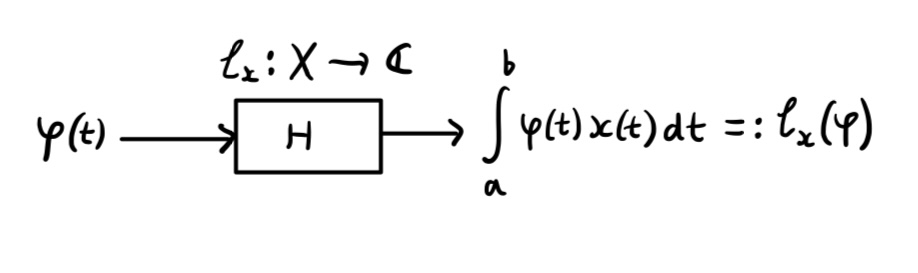
\includegraphics[width=0.8\linewidth]{figures/Funktionale_2 copy.jpg}
    \end{center}
\end{frame}

\begin{frame}{Funktionale}
    \begin{center}
        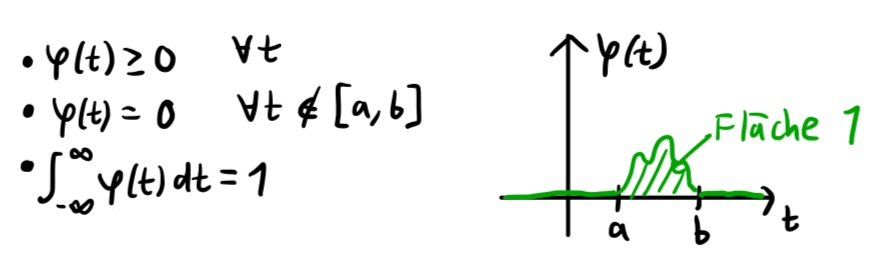
\includegraphics[width=0.8\linewidth]{figures/Funktionale_3.jpg}
    \end{center}
    \begin{itemize}
        \item \textbf{Mittelwertsatz} der Integration: 
        \item[] $\exists \xi \in [a,b], \text{ sodass }  \ell_x(\varphi) = \displaystyle\int_a^b \varphi(t)x(t)dt = x(\xi)\displaystyle\int_a^b \varphi(t)dt$
    \end{itemize}
\end{frame}

\begin{frame}{Deltafolgen}
    \begin{itemize}
        \item Eine Deltafolge $\delta_n(t)$ hat folgende Eigenschaften:
        \item[] 
        \item[1.]  $\delta_n(t) \begin{cases}
        \geq 0, \hspace{20pt} \forall t \in I_n = [a_n, b_n]\\
        = 0, \hspace{20pt} \forall t \notin I_n
        \end{cases}$
    \end{itemize}
    \begin{center}
        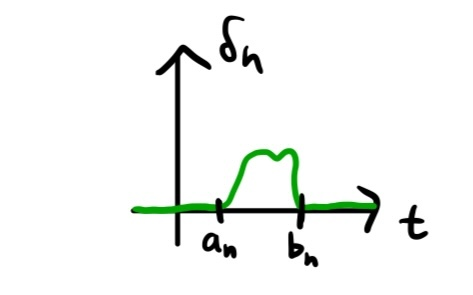
\includegraphics[width=0.4\linewidth]{figures/Deltafolge_3.jpg}
    \end{center}
\end{frame}

\begin{frame}{Deltafolgen}
    \begin{itemize}
        \item[2.] Die Intervalle $I_n$ bilden eine \textbf{Intervallverschachtelung} für $t_0 \in \mathbb{R}$, d.h. die Intervalle, auf denen $\delta_n(t) \geq 0$ werden immer schmäler: $ \hspace{12pt} a_1 \leq a_2 \leq \dots \leq t_0 \leq \dots \leq b_2 \leq b_1$
        \item[] 
        \item[] $\displaystyle\lim_{n \to \infty}a_n = \displaystyle\lim_{n \to \infty}b_n = t_0$
    \end{itemize}
    \begin{center}
        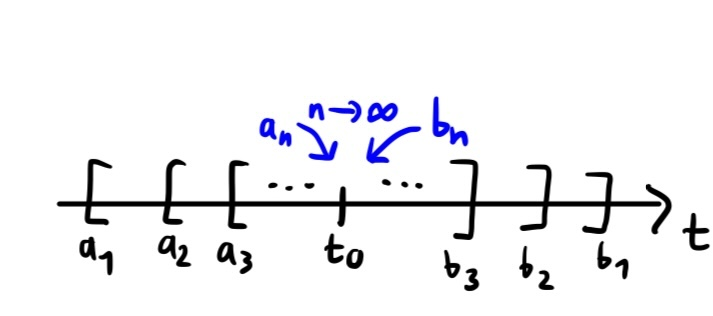
\includegraphics[width=0.6\linewidth]{figures/Deltafolge_4.jpg}
    \end{center}
\end{frame}

\begin{frame}{Deltafolgen}
    \begin{itemize}
        \item[3.]  \textbf{Normierung}: $\forall n$ gilt $\displaystyle\int_{-\infty}^\infty \delta_n(t)\text{d}t = \displaystyle\int_{a_n}^{b_n}\delta_n(t)\text{d}t = 1$
    \end{itemize}
    \begin{center}
        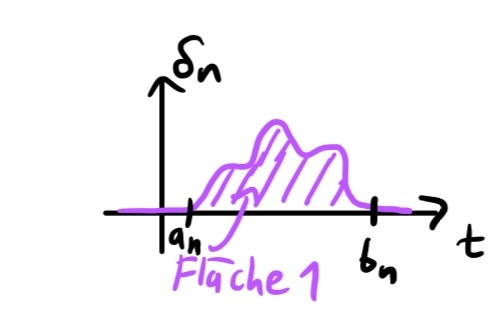
\includegraphics[width=0.4\linewidth]{figures/Deltafolge_5.jpg}
    \end{center}
\end{frame}

\begin{frame}{Deltafolgen}
    \begin{center}
        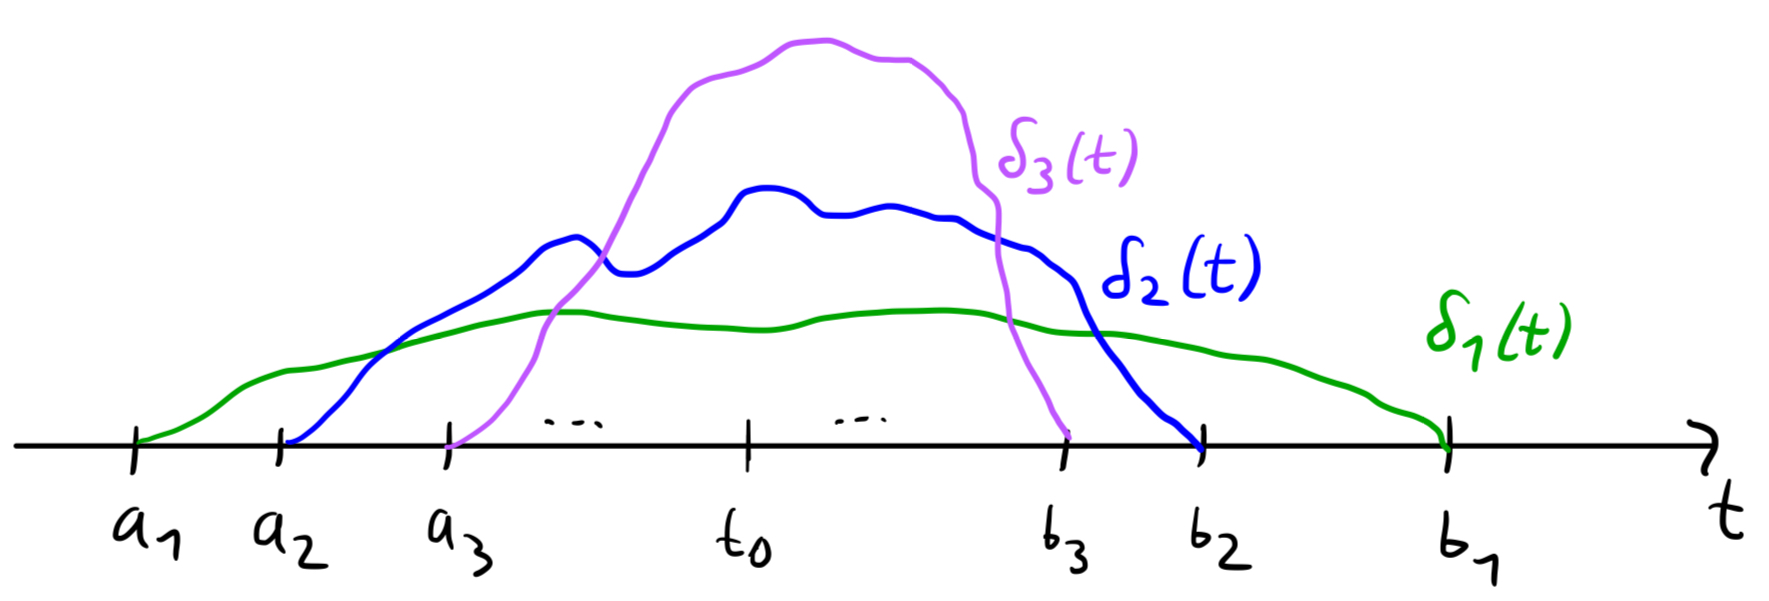
\includegraphics[width=0.9\linewidth]{figures/Deltafolge_2.jpg}
    \end{center}
\end{frame}

\begin{frame}{Dirac-Delta}
    \begin{itemize}
        \item Wir nehmen den Grenzwert für $n \to \infty$ und erhalten die \textbf{Dirac-Delta} "Funktion":
        $$\delta_{t_0}(t) := \lim_{n \to \infty} \delta_n(t) \; \begin{cases}
        \to \infty, \hspace{20pt} t = t_0\\
        = 0, \hspace{28pt} t \neq t_0
        \end{cases} = \delta(t-t_0)$$
        \item Eigenschaften: Breite $0$, Höhe $\to \infty$ und Fläche $1$
    \end{itemize}
\end{frame}

\begin{frame}{Deltafunktion}
    \begin{itemize}
        \item Wir betrachten die Funktion:
        $$\delta(t, \varepsilon) = \begin{cases}
        \frac{1}{2\varepsilon} \hspace{12pt} |t|\leq \varepsilon\\
        0, \hspace{20pt} \text{sonst}
    \end{cases}$$
    \item[] 
    \item $\ell_x(\delta(t, \varepsilon)) = \displaystyle\int_{-\infty}^{\infty} x(t) \delta(t, \varepsilon)\text{d}t = x(\xi) \displaystyle\int_{-\varepsilon}^\varepsilon \delta(t, \varepsilon)\text{d}t = x(\xi)$
    \item[] 
    \item Wir lassen $\varepsilon \to \infty$, dann $\xi \to 0$ und somit $\displaystyle\lim_{\varepsilon \to 0} \ell_x(\delta(t, \varepsilon)) = x(0)$. Man schreibt $\delta(t) = \displaystyle\lim_{\varepsilon \to 0}\delta(t,\varepsilon)$
    \end{itemize}
\end{frame}

\begin{frame}{Deltafunktion}
    \begin{center}
        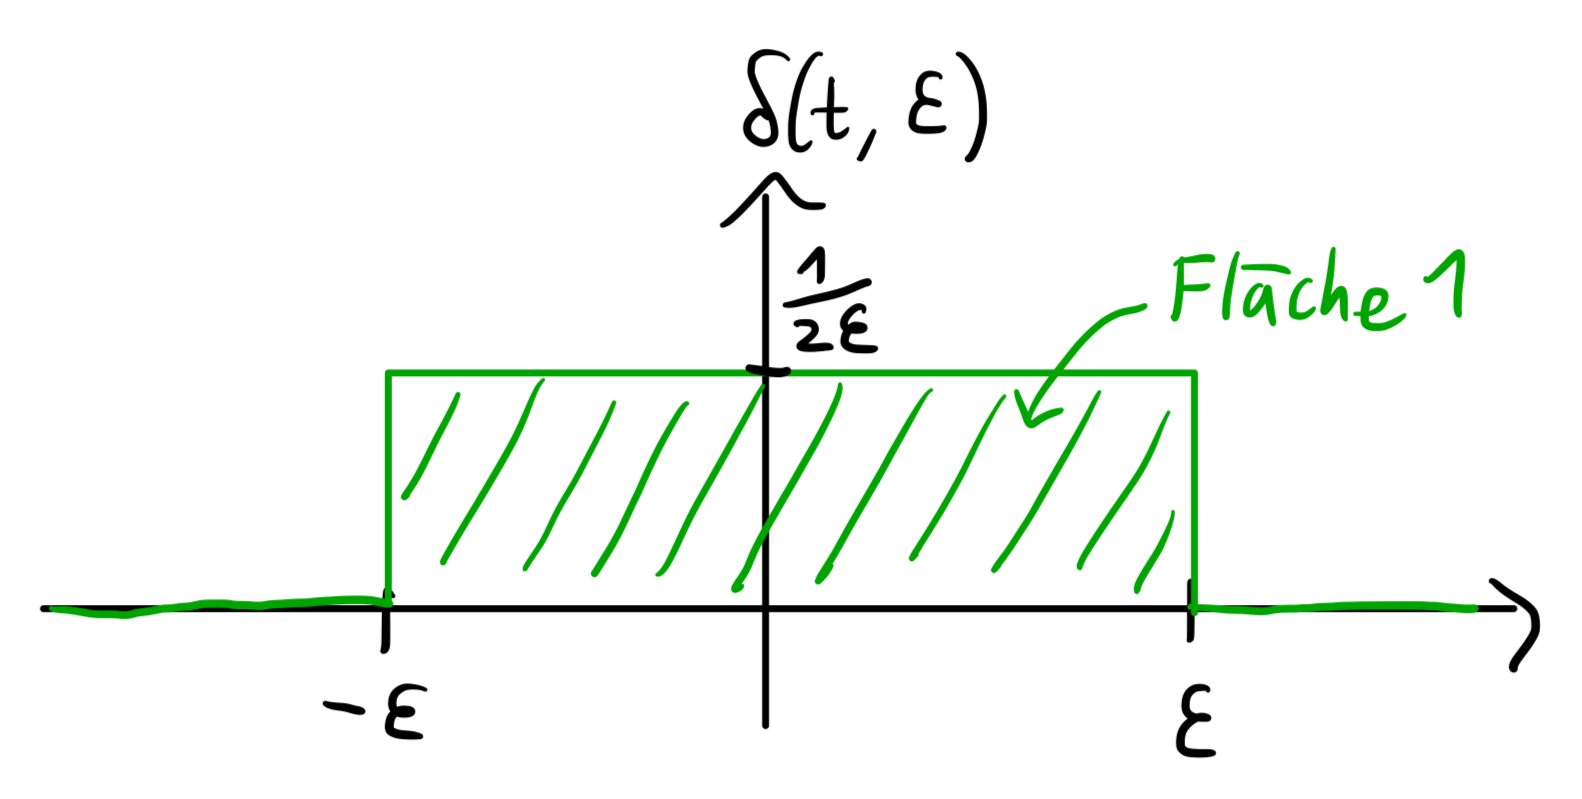
\includegraphics[width=0.4\linewidth]{figures/Deltafunktion_1.jpg}
        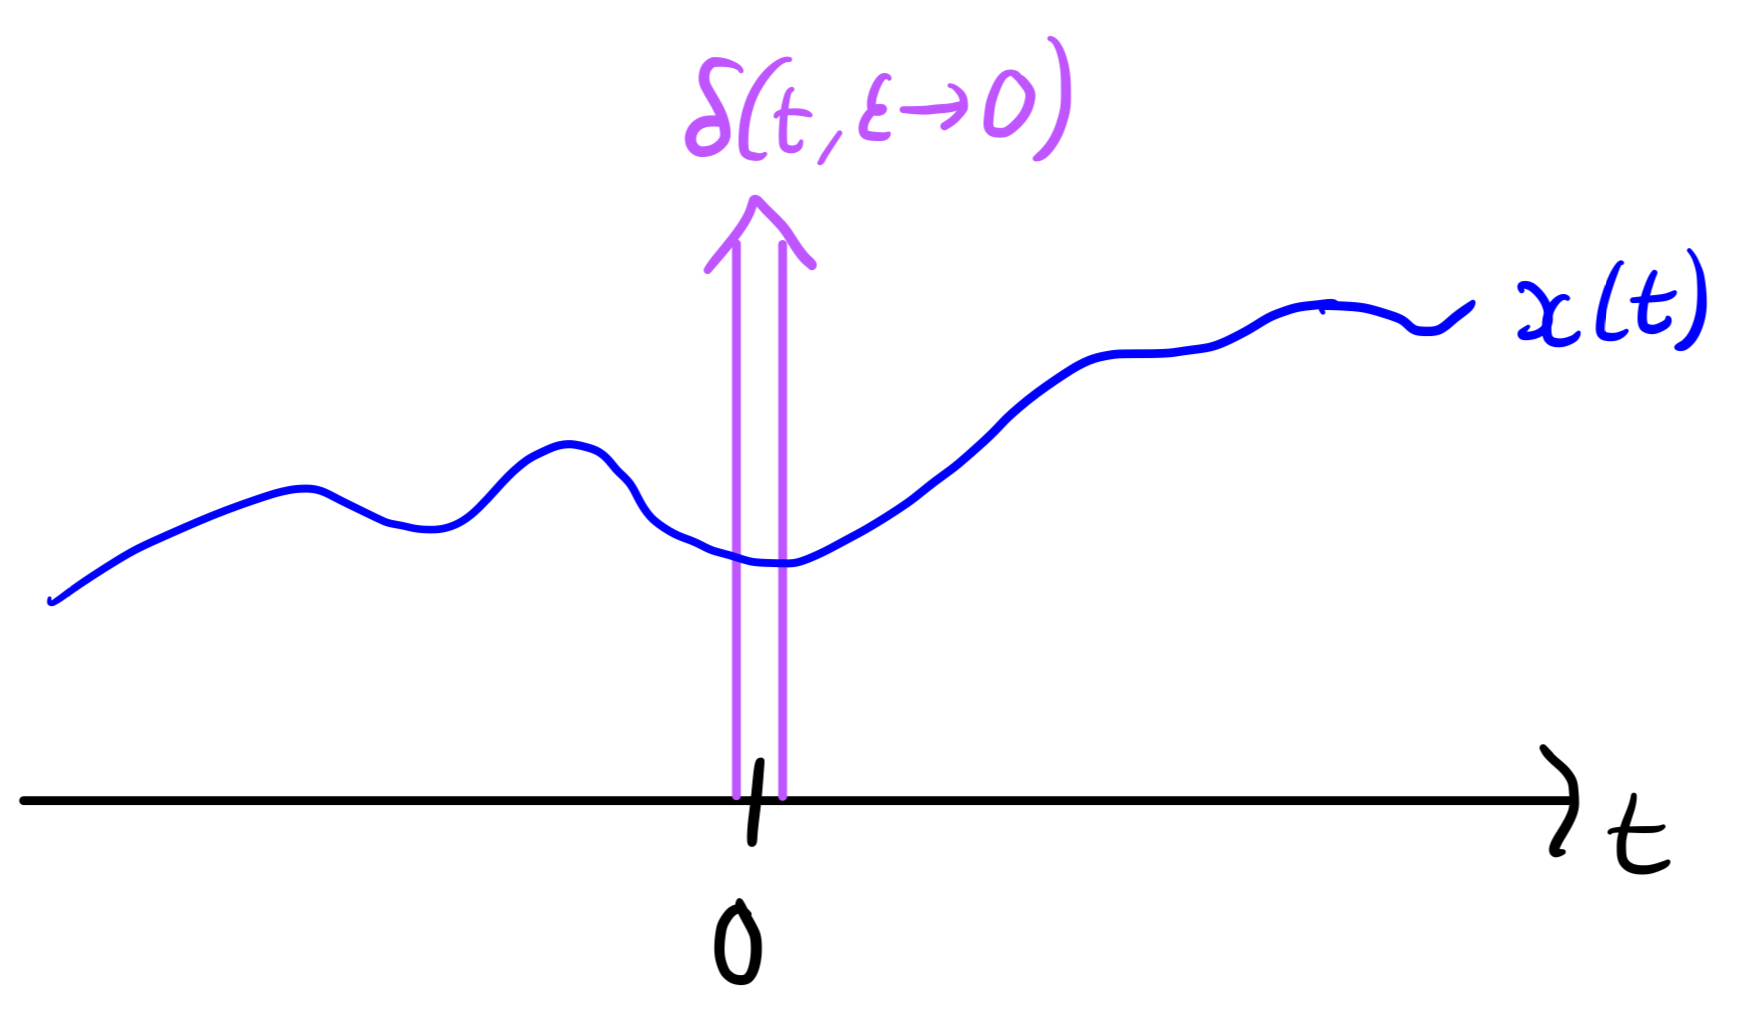
\includegraphics[width=0.4\linewidth]{figures/Deltafunktion_2.jpg}
    \end{center}
    $$\implies \delta(t)x(t) = \delta(t)x(0), \hspace{4pt} \text{ dann } $$
    $$\hspace{4pt} \int_{-\infty}^{\infty} x(t)\delta(t) \text{d}t = \int_{-\infty}^{\infty} x(0)\delta(t) \text{d}t = x(0)\int_{-\infty}^{\infty}\delta(t) \text{d}t = x(0)$$
\end{frame}

\begin{frame}{Eigenschaften der Deltafunktion}
    \begin{itemize}
        \item[1.] \textbf{Symmetrie}: 
        \item[] $\delta(t) = \delta(-t)$
        \item[] $\delta(t-t_0) = \delta(t_0 - t)$
        \item[] 
        \item[2.] \textbf{Multiplikation mit einer Funktion}: \item[] $x(t)\delta(t) = x(0)\delta(t)$
        \item[] $x(t)\delta(t-t_0)=x(t_0)\delta(t-t_0)$
    \end{itemize}
\end{frame}

\begin{frame}{Eigenschaften der Deltafunktion}
    \begin{itemize}
        \item[3.] \textbf{Siebeigenschaft}: 
        \item[] $\displaystyle\int_{-\infty}^{\infty}\delta(t)x(t)\text{d}t = x(0)$
        \item[] $\displaystyle\int_{-\infty}^{\infty}\delta(t-t_0)x(t)\text{d}t = x(t_0)$
    \end{itemize}
\end{frame}

\begin{frame}{Eigenschaften der Deltafunktion}
    \begin{itemize}
        \item[4.] \textbf{Verschiebung/Skalierung des Parameters}:
    \item[] $\delta(at + b) = \displaystyle\frac{1}{|a|}\delta\left(t + \displaystyle\frac{b}{a} \right)$
    \end{itemize}
\end{frame}

\begin{frame}{Eigenschaften der Deltafunktion}
    \begin{itemize}
        \item[5.] \textbf{Die $\delta-$Funktion ist das Einselement der Faltung}:
        \item[] $(x \ast \delta)(t) = \displaystyle\int_{-\infty}^\infty x(t-\tau)\delta(\tau)\text{d}\tau = x(t)$
        \item[] $(x \ast \delta(\cdot - t_0))(t) = x(t - t_0)$
    \end{itemize}
\end{frame}

\begin{frame}{Eigenschaften der Deltafunktion}
    \begin{itemize}
        \item[6.] \textbf{Einheitssprungfunktion}:
        \item[] $\displaystyle\int_{-\infty}^t \delta(\tau) \text{d}\tau = \sigma(t)$
    \end{itemize}
\end{frame}

\begin{frame}{Ableitung verallgemeinerter Funktionen}
    \begin{itemize}
        \item \textbf{Notation}:
        \item[] $D =$ Ableitungsoperator
        \item[] $x'(t) =$ konventionelle Definition der Ableitung einer stetigen, differenzierbaren Funktion (Vgl. Analysis 1)
        \item[]  $t_0 =$ eine Sprungstelle von $x(t)$
        \item[] 
    \end{itemize}
    $$(Dx)(t) = x'(t) + (x(t_0^+)- x(t_0^-))\delta(t-t_0)$$
\end{frame}

\begin{frame}{Bemerkung}
    \begin{itemize}
        \item Impulsantwort $h(t) := (H \delta)(t)$
        \item Sprungantwort $a(t) := (H \sigma)(t)$
        \item[] 
    \end{itemize}
\fcolorbox{darkblue}{lightblue}{%
\parbox{\dimexpr\linewidth-2\fboxsep-2\fboxrule\relax}{
    \begin{center}
        Da $\displaystyle\frac{\text{d}\sigma(t)}{\text{d}t} = \delta(t) \hspace{10pt}$ haben wir $ \hspace{10pt} \displaystyle\frac{\text{d}a(t)}{\text{d}t} = h(t)$
    \end{center}
}}%
\end{frame}

\begin{frame}{Aufgaben}
    \begin{itemize}
        \item \textbf{Aufgabe 50}
        \item[] 
        \item \textbf{Aufgabe 51}
    \end{itemize}
\end{frame}

\begin{frame}{Analoge Lineare Systeme im Frequenzbereich}
\begin{itemize}
    \item \textbf{Motivation}
\end{itemize}
\begin{center}
     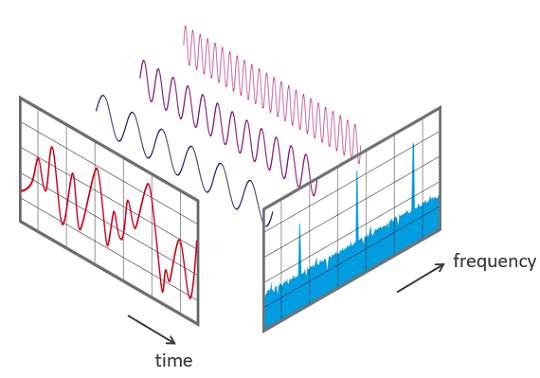
\includegraphics[width=0.65\linewidth]{figures/Zeit_und_Frequenzbereich.png}
\end{center} 
\end{frame}

\begin{frame}{Fouriertransformation}
    \begin{itemize}
    \item \textbf{Fouriertransformation (FT)}:
    \item[] \fcolorbox{darkblue}{lightblue}{%
\parbox{\dimexpr\linewidth-2\fboxsep-2\fboxrule\relax}{
    $$\hat{x}(f) = (\mathcal{F}x)(f) = \int_{-\infty}^{\infty}x(t)e^{-2\pi i f t}\text{d}t$$
}}%
    \item[] 
    \item[] 
    \item \textbf{Inverse Fouriertransformation (IFT)}:
    \item[] \fcolorbox{darkblue}{lightblue}{%
\parbox{\dimexpr\linewidth-2\fboxsep-2\fboxrule\relax}{
    $$x(t) = (\mathcal{F}^{-1}\hat{x})(t) = \int_{-\infty}^{\infty}\hat{x}(f)e^{2\pi i f t}\text{d}f$$
}}%
\end{itemize}
\end{frame}

\begin{frame}{Fouriertransformation: Hinweise}
    \begin{itemize}
        \item KomA/NuS 2: FT und IFT waren definiert als:
$$\hat{x}(\omega) = \int_{-\infty}^{\infty} x(t) e^{-i\omega t}\text{d}t, \hspace{20pt} x(t)=\frac{1}{2\pi} \int_{-\infty}^{\infty} \hat{x}(\omega)e^{i\omega t} \text{d}\omega$$
    \item In SST1 haben wir $t$ und $f$ als Parameter  anstatt $t$ und $\omega$
    \item[] 
    \item $\omega = 2\pi f \implies \text{d}\omega = 2\pi \text{d}f \implies$ kein Vorfaktor $1/(2\pi)$ in IFT
    \end{itemize}
\end{frame}

\begin{frame}{Fouriertransformation: Hinweise}
    \begin{itemize}
        \item Die Fouriertransformation ist eine \textbf{lineare Abbildung}. (\textbf{Additivität} \& \textbf{Homogenität})
        \item[] 
        \item \alert{Berechnet die FT und IFT mithilfe der Transformationstabellen.}
        \item[] 
        \item An der Prüfung muss man eigentlich nie die Integrale der FT berechnen. Es gibt immer einen Kunstgriff, nachdem man die FT von der Tabelle ablesen kann.
    \end{itemize}
\end{frame}

\begin{frame}{Aufgaben}
    \begin{itemize}
        \item \textbf{Aufgabe 58.b)}
        \item[] 
        \item \textbf{Aufgabe 60.b)}
        \item[] 
        \item \textbf{Aufgabe 64.b)}
    \end{itemize}
\end{frame}

\begin{frame}{Dualität der Fouriertransformation}
    \includegraphics[width=0.45\linewidth]{figures/dualität_1.png}
    \includegraphics[width=0.45\linewidth]{figures/dualität_2.png}
\end{frame}

\begin{frame}{Beispiel}
    
\end{frame}

\begin{frame}{Parseval und Plancherel}
    \fcolorbox{darkblue}{lightblue}{%
    \parbox{\dimexpr\linewidth-2\fboxsep-2\fboxrule\relax}{
    \begin{center}
        \textbf{Plancherelsche Identität:}
    \end{center}
    $$\langle x, y \rangle = \int_{-\infty}^{\infty} x(t)y^\ast (t)\text{d}t = \int_{-\infty}^{\infty}\hat{x}(f)\hat{y}(f)\text{d}f = \langle \hat{x}, \hat{y} \rangle$$
    \begin{center}
        \textbf{Parsevalsche Beziehung:}
    \end{center}
    $$||x||^2 = \langle x, x \rangle = \int_{-\infty}^{\infty} |x(t)|^2\text{d}t = \int_{-\infty}^{\infty}|\hat{x}(f)|^2\text{d}f = \langle \hat{x}, \hat{x} \rangle = ||\hat{x}||^2$$
    }}
\end{frame}

\begin{frame}{Plancherelsche Identität}
    \begin{itemize}
    \item \textbf{Theorem}: Wenn $f,g \in L^2(\mathbb{R})$, dann gilt $\langle x, y\rangle = \langle \hat{x}, \hat{y}\rangle$
    \item[] $\implies \mathcal{F}$ ist längenerhaltend und winkelerhaltend
    \item \textbf{Beweis}:
    \item[]
    \item[]
    \item[]
    \item[]
    \item[]
    \item[]
    \item[]
\end{itemize}
\end{frame}

\begin{frame}{Aufgaben}
    \begin{itemize}
        \item \textbf{Aufgabe 66}
        \item[]
        \item \textbf{Prüfungsaufgabe: Sommer 2020, Aufgabe 4.a)}
    \end{itemize}
\end{frame}

\end{document}
